% standard beamer lecture template for slides
% by Derek Huang
\documentclass{beamer}
\usepackage[utf8]{inputenc}
\usepackage{algorithm2e, amsmath, amssymb, amsfonts, graphicx}
% allow section.equation numbering
\numberwithin{equation}{section}
% use boadilla theme
\usetheme{Boadilla}
% remove navigation symbols
\usenavigationsymbolstemplate{}
% get numbered figure captions
\setbeamertemplate{caption}[numbered]
% changes itemize to circle + other things
\useoutertheme{split}
\useinnertheme{circles}

% command for the title string. change for each lecture
\newcommand{\lecturetitle}{Intro to Optimization, Part 1}
% allow automatic alert-highlighted references and hyperlinks
\newcommand{\aref}[1]{\alert{\ref{#1}}}
\newcommand{\ahref}[2]{\href{#1}{\alert{#2}}}
% title page stuff. brackets content displayed in footer bar
\title[\lecturetitle]{\lecturetitle}
% metadata. content in brackets is displayed in footer bar
\author[Derek Huang (BAC Advanced Team)]{Derek Huang}
\institute{BAC Advanced Team}
\date{April 8, 2021}

% change "ball" bullet to numbered bullet and section title for section
\setbeamertemplate{section in toc}{\inserttocsectionnumber.~\inserttocsection}
% change ball to gray square (copied from stackoverflow; \par needed for break)
\setbeamertemplate{subsection in toc}{        
    \hspace{1.2em}{\color{gray}\rule[0.3ex]{3pt}{3pt}}~\inserttocsubsection\par}
% use default enumeration scheme
\setbeamertemplate{enumerate items}[default]
% required line that fixes the problem of \mathbf, \bf not working in beamer
% for later (post-2019) TeX Live installations. see the issue on GitHub:
% https://github.com/josephwright/beamer/issues/630
\DeclareFontShape{OT1}{cmss}{b}{n}{<->ssub * cmss/bx/n}{}

\begin{document}

% title slide
\begin{frame}
    \titlepage
    \centering
    % relative path may need to be updated depending on .tex file location
    
\includegraphics[scale = 0.1]{../bac_logo1.png}
\end{frame}

% table of contents slide
\begin{frame}{Overview}
    \tableofcontents
\end{frame}

\section{Convex optimization}

\begin{frame}{Motivation}
    \begin{itemize}
        \item
        Let $ \mathbf{X} \in \mathbb{R}^{N \times d} $ be the input matrix,
        $ \mathbf{y} \in \mathbb{R}^N $ the response vector. Consider
        fitting a linear regression model s.t. we minimize the
        absolute value of the residuals. Optimal $ \hat{\mathbf{w}} \in
        \mathbb{R}^d $, $ \hat{b} \in \mathbb{R} $ solve
        \begin{equation*}
            \begin{array}{ll}
                \displaystyle\min_{\mathbf{w}, b} &
                    \Vert\mathbf{y} - \mathbf{Xw} - b\mathbf{1}\Vert_1
            \end{array}
        \end{equation*}

        \item
        Model parameter estimation is an optimization problem.

        \item
        Quite hard to solve. May be recast as the linear program (LP)
        \cite{bv_convex_opt}
        \begin{equation*}
            \begin{array}{ll}
                \displaystyle\min_{\mathbf{w}, b, \mathbf{t}} &
                    \mathbf{1}^\top\mathbf{t} \\
                \text{s.t.} &
                    -\mathbf{t} \preceq \mathbf{y} - \mathbf{Xw} - b\mathbf{1}
                    \preceq \mathbf{t} \\
                & \mathbf{t} \succeq \mathbf{0}
            \end{array}
        \end{equation*}
        Here $ \mathbf{t} \in \mathbb{R}^N $. Algorithms for solving LPs
        are quite reliable \cite{bv_convex_opt}.
    \end{itemize}
\end{frame}

\subsection{Convex sets and functions}

\begin{frame}{Convex sets and functions}
    \begin{itemize}
        \item
        Optimization problems broadly categorized as convex vs. nonconvex
        $ \Rightarrow $ we need to know what convexity means.

        \item
        \textit{Definition.} Let $ \mathbf{x}_1, \mathbf{x}_2 \in
        \mathbb{R}^n $, $ \mathbf{x}_1 \ne \mathbf{x}_2 $. The \textit{line}
        passing through points $ \mathbf{x}_1, \mathbf{x}_2 $ is
        $ \{\theta\mathbf{x}_1 + (1 - \theta)\mathbf{x}_2 :
        \theta \in \mathbb{R}\} $. The \textit{line segment} connecting
        points $ \mathbf{x}_1, \mathbf{x}_2 $ is $ \{\theta\mathbf{x}_1 +
        (1 - \theta) \mathbf{x}_2 : \theta \in [0, 1]\} $
        \cite{bv_convex_opt}.
    \end{itemize}
    \begin{figure}
        \centering
        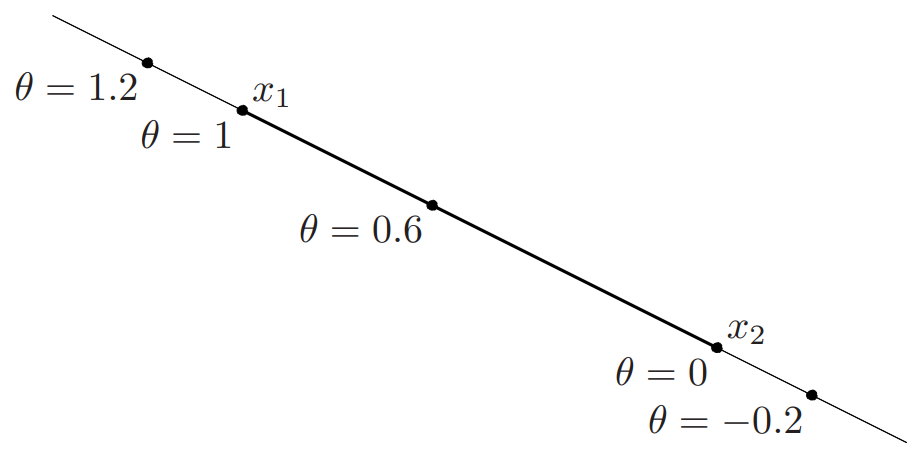
\includegraphics[scale = 0.3]{bv_fig_2.1.png}
        % remove excess space
        \vspace{-10 pt}
        \caption{
            The $ \mathbf{x}_1, \mathbf{x}_2 $ line and line segment
            parametrized by $ \theta $\footnote{
                Figure 2.1 from Boyd and Vandenberghe's
                \textit{Convex Optimization}.
            }.
        }
    \end{figure}
\end{frame}

\begin{frame}{Convex sets and functions}
    \begin{itemize}
        \item
        \textit{Definition.} A set $ C \subseteq \mathbb{R}^n $ is
        \textit{affine} if $ \forall \mathbf{x}, \mathbf{y} \in C $,
        $ \alpha \in \mathbb{R} $, $ \alpha\mathbf{x} + (1 - \alpha)\mathbf{y}
        \in C $, i.e. $ C $ contains the $ \mathbf{x}, \mathbf{y} $ line.

        \item
        \textit{Definition.} Let $ C \subseteq \mathbb{R}^n $. The
        \textit{affine hull} of $ C $, denoted $ \operatorname{aff} C $, is
        $ \operatorname{aff} C \triangleq \{
            \sum_{i = 1}^k\theta_i\mathbf{x}_i : \mathbf{x}_1, \ldots
            \mathbf{x}_k \in C, \theta_1, \ldots \theta_k \in \mathbb{R},
            \sum_{i = 1}^k\theta_i = 1
        \} $ \cite{bv_convex_opt}.

        \item
        \textit{Definition.} A set $ C \subseteq \mathbb{R}^n $ is
        \textit{convex} if $ \forall \mathbf{x}, \mathbf{y} \in C $,
        $ \alpha \in [0, 1] $,
        $ \alpha\mathbf{x} + (1 - \alpha)\mathbf{y} \in C $, i.e. $ C $
        contains the $ \mathbf{x}, \mathbf{y} $ line segment.
    \end{itemize}
    \begin{figure}
        \centering
        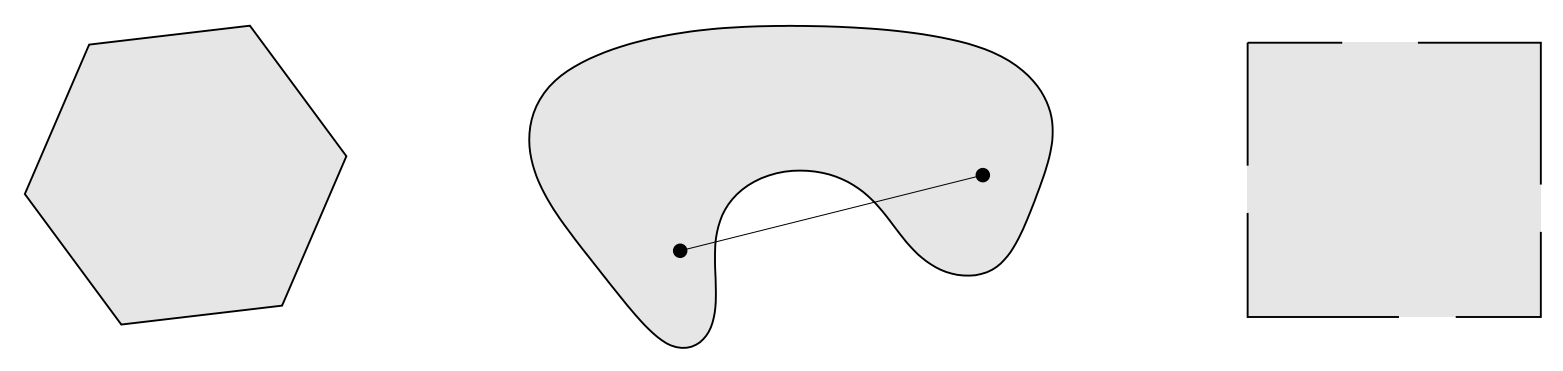
\includegraphics[scale = 0.2]{bv_fig_2.2.png}
        % remove excess space
        \vspace{-10 pt}
        \caption{
            Convex and nonconvex sets. Only the leftmost set is
            convex\footnote{
                Figure 2.2 from Boyd and Vandenberghe's
                \textit{Convex Optimization}.
            }.
        }
        % remove excess space
        \vspace{-10 pt}
    \end{figure}
    \begin{itemize}
        \item
        \textit{Definition.} Let $ C \subseteq \mathbb{R}^n $. The
        \textit{convex hull} of $ C $, denoted $ \operatorname{conv} C $, is
        $ \operatorname{conv} C \triangleq \{
            \sum_{i = 1}^k\theta_i\mathbf{x}_i : \mathbf{x}_1, \ldots
            \mathbf{x}_k \in C, \theta_1, \ldots \theta_k \in [0, 1],
            \sum_{i = 1}^k\theta_i = 1        
        \} $.
    \end{itemize}
    % adjust spacing since there is a footnote
    \bigskip
\end{frame}

\begin{frame}{Convex sets and functions}
    \begin{itemize}
        \item
        If $ C $ affine, then $ \operatorname{aff} C = C $, while if $ C $
        convex, then $ \operatorname{conv} C = C $.
    \end{itemize}
    \begin{figure}
        \centering
        % remove excess space
        \vspace{-3 pt}
        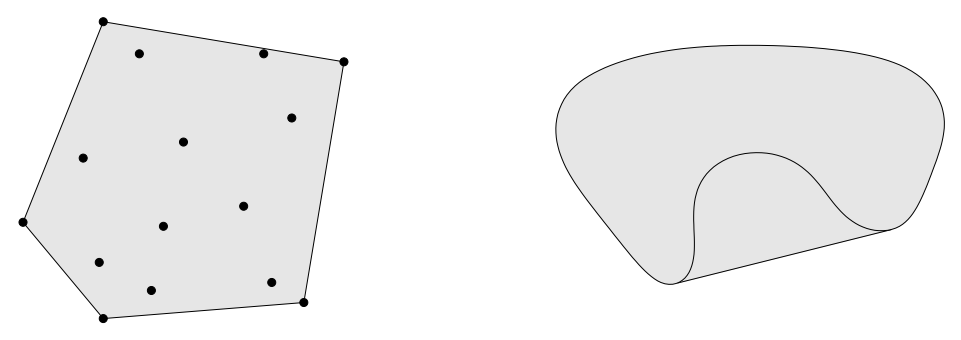
\includegraphics[scale = 0.24]{bv_fig_2.3.png}
        % remove excess space
        \vspace{-10 pt}
        \caption{
            Examples of $ \mathbb{R}^2 $ convex hulls\footnote{
                Figure 2.3 from Boyd and Vandenberghe's
                \textit{Convex Optimization}.
            }.
        }
        % remove excess space
        \vspace{-10 pt}
    \end{figure}
    \begin{itemize}
        \item
        \textit{Definition.} Let $ C \subseteq \mathbb{R}^n $. The
        \textit{relative interior} of $ C $, denoted
        $ \operatorname{relint} C $, is $ \operatorname{relint} C \triangleq 
        \{\mathbf{x} \in C : B(\mathbf{x}, r) \cap \operatorname{aff} C
        \subseteq C, r \in (0, \infty)\} $ \cite{bv_convex_opt}. Here
        $ B(\mathbf{x}, r) \triangleq \{\mathbf{x}' \in \mathbb{R}^n :
        \Vert\mathbf{x}' - \mathbf{x}\Vert \le r\} $ for some norm
        $ \Vert\cdot\Vert $\footnote{
            All norms define the same relative interior \cite{bv_convex_opt}.        
        }.

        \item
        \textit{Definition.} $ f : \mathcal{M} \rightarrow
        \mathbb{R} $, $ \mathcal{M} \subseteq \mathbb{R}^n $, is
        \textit{convex} if $ \mathcal{M} $ convex and if
        $ \forall \mathbf{x}, \mathbf{y} \in \mathcal{M} $,
        $ \forall \alpha \in [0, 1] $,
        $ f(\alpha\mathbf{x} + (1 - \alpha)\mathbf{y}) \le
        \alpha f(\mathbf{x}) + (1 - \alpha)f(\mathbf{y}) $.

        \item
        \textit{Definition.} $ f : \mathcal{M} \rightarrow \mathbb{R} $ is
        \textit{concave} if $ -f $ is convex.
    \end{itemize}

    % spacing for footnote
    \bigskip
\end{frame}

\begin{frame}{Convex sets and functions}
    \begin{itemize}
        \item
        Affine and linear functions are both convex and concave.
    \end{itemize}
    \begin{figure}
        \centering
        % remove extra space
        \vspace{-3 pt}
        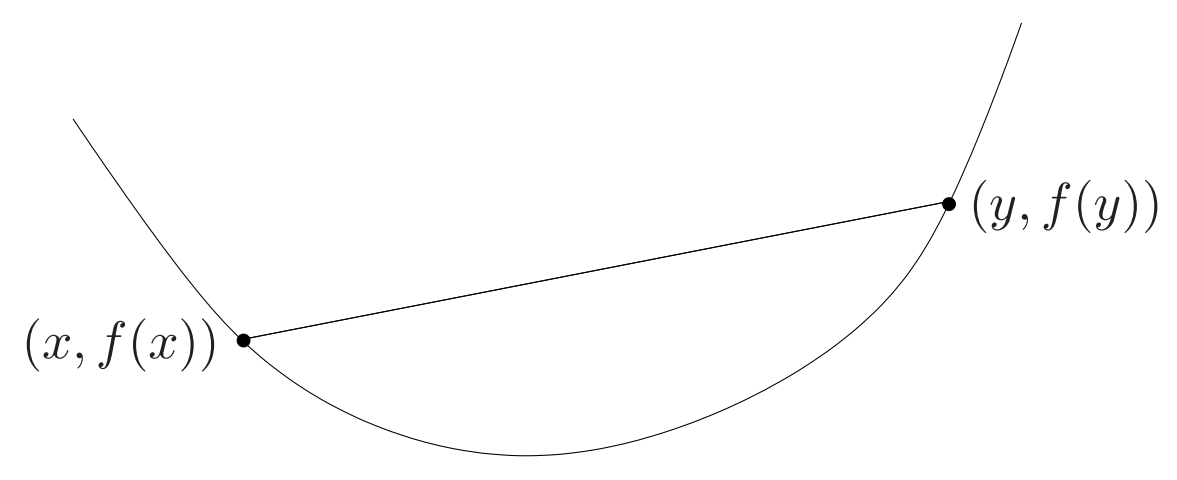
\includegraphics[scale = 0.24]{bv_fig_3.1.png}
        % remove extra space
        \vspace{-5 pt}
        \caption{Graph of a convex function\footnote{
            Figure 3.1 from Boyd and Vandenberghe's
            \textit{Convex Optimization}.
        }. }
        % remove excess space
        \vspace{-10 pt}
    \end{figure}
    \begin{itemize}
        \item
        \textit{Examples.}
        \begin{itemize}
            \item
            \textit{Exponential.} $ \forall a \in \mathbb{R} $, $ e^{ax} $
            convex on $ \mathbb{R} $ \cite{bv_convex_opt}.

            \item
            \textit{Powers.} $ x^a $ convex on $ (0, \infty) $ if
            $ a \in (\infty, 0] \cup [1, \infty) $, concave if
            $ a \in [0, 1] $. $ \forall a \in [1, \infty) $, $ |x|^a $ convex
            on $ \mathbb{R} $ \cite{bv_convex_opt}.

            \item
            \textit{Logarithms.} $ \log x $ concave on $ (0, \infty) $.

            \item
            \textit{Norms.} Any norm on $ \mathbb{R}^n $ is convex
            \cite{bv_convex_opt}, e.g. $ \ell^p $-norm.
        \end{itemize}
    \end{itemize}

    % spacing for footnote
    \bigskip
\end{frame}

\begin{frame}{Convex sets and functions}
    \begin{itemize}
        \item
        \textit{Theorem.} Let $ f : \mathcal{M} \rightarrow \mathbb{R} $ be
        differentiable $ \forall \mathbf{x} \in \mathcal{M} $. $ f $
        convex $ \Leftrightarrow \mathcal{M} $ convex, $ \forall \mathbf{x},
        \mathbf{y} \in \mathcal{M} $, $ f(\mathbf{y}) \ge f(\mathbf{x}) +
        \nabla f(\mathbf{x})^\top(\mathbf{y} - \mathbf{x}) $
        \cite{bv_convex_opt}.
    \end{itemize}
    \begin{figure}
        \centering
        % remove extra space
        \vspace{-5 pt}
        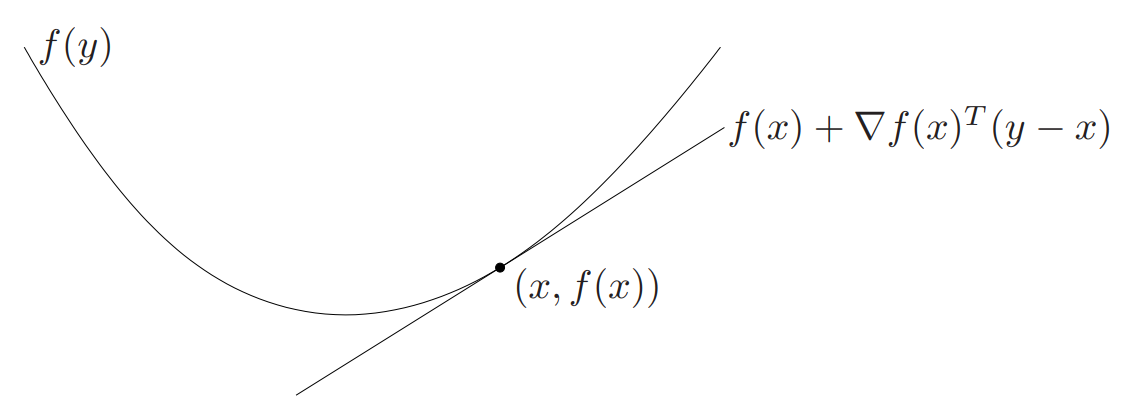
\includegraphics[scale = 0.3]{bv_fig_3.2.png}
        % remove extra space
        \vspace{-10 pt}
        \caption{Convex function bounded below by tangent line\footnote{
            Figure 3.2 from Boyd and Vandenberghe's
            \textit{Convex Optimization}.
        }. }
        % remove excess space
        \vspace{-15 pt}
    \end{figure}
    \begin{itemize}
        \item
        \textit{Theorem.} Let $ f : \mathcal{M} \rightarrow \mathbb{R} $ be
        twice differentiable $ \forall \mathbf{x} \in \mathcal{M} $.
        $ f $ convex $ \Leftrightarrow \mathcal{M} $ convex, $ \forall
        \mathbf{x} \in \mathcal{M} $, $ \nabla^2f(\mathbf{x}) \succeq
        \mathbf{0} $ \cite{bv_convex_opt}.

        \item
        \textit{Remark.} If $ \mathcal{M} \subseteq \mathbb{R} $ convex,
        reduces to $ \forall x \in \mathcal{M}, f''(x) \ge 0 $.
    \end{itemize}

    % spacing for footnote
    \medskip

\end{frame}

\subsection{Optimization problems}

\begin{frame}{Optimization problems}
    \begin{itemize}
        \item
        \textit{Definition.} Let $ \mathcal{M}_f, \mathcal{M}_\mathbf{u},
        \mathcal{M}_\mathbf{v} \subseteq \mathbb{R}^n $. For
        $ f: \mathcal{M}_f \rightarrow \mathbb{R} $, $ \mathbf{u} :
        \mathcal{M}_\mathbf{u} \rightarrow \mathbb{R}^p $,
        $ \mathbf{v} : \mathcal{M}_\mathbf{v} \rightarrow \mathbb{R}^q $, a
        \textit{standard form} optimization problem is\footnote{
            Assume the problem is well-defined, i.e. \textit{feasible}
            (solvable) and bounded below.
        }
        \cite{bv_convex_opt}
        \begin{equation} \label{opt_prob_std}
            \begin{array}{ll}
                \displaystyle\min_\mathbf{x} & f(\mathbf{x}) \\
                \text{s.t.} & \mathbf{u}(\mathbf{x}) \preceq \mathbf{0} \\
                & \mathbf{v}(\mathbf{x}) = \mathbf{0}
            \end{array}
        \end{equation}
        $ \mathbf{x} \in \mathbb{R}^n $ is the \textit{optimization
        variable} \cite{bv_convex_opt}. $ \mathbf{u} \triangleq
        [ \ u_1 \ \ldots \ u_p \ ]^\top $ gives $ p $ \textit{inequality
        constraints}, $ \mathbf{v} \triangleq [ \ v_1 \ \ldots \ v_q \ ]^\top $
        gives $ q $ \textit{equality constraints}.

        \item
        \textit{Definition.} The \textit{domain} of (\aref{opt_prob_std}) is
        $ \tilde{\mathcal{M}} \triangleq \mathcal{M}_f \cap
        \mathcal{M}_\mathbf{u} \cap \mathcal{M}_\mathbf{v} \ne \emptyset $
        \cite{bv_convex_opt}.

        \item
        Problem is \textit{constrained} if no constraints,
        \textit{unconstrained} otherwise. Note maximization of $ f $ 
        equivalent to minimization of $ -f $.

        \item
        \textit{Definition.} (\aref{opt_prob_std}) is a
        \textit{convex optimization problem} if functions
        $ f, u_1, \ldots u_p $ are convex and functions $ v_1, \ldots v_q $
        are affine \cite{bv_convex_opt}.
    \end{itemize}

    % spacing for footnote
    \medskip
\end{frame}

\begin{frame}{Optimization problems}
    \begin{itemize}
        \item
        \textit{Examples.}
        \begin{itemize}
            \item
            \textit{Weighted linear least squares.} Let $ \mathbf{\Gamma}
            \triangleq \operatorname{diag}(\gamma_1, \ldots \gamma_N) \succ
            \mathbf{0} \in \mathbb{R}^{N \times N} $ be the data weighting
            matrix. The unconstrained problem to solve is
            \begin{equation*}
                \begin{array}{ll}
                    \displaystyle\min_{\mathbf{w}, b} &
                    \Vert
                        \mathbf{\Gamma}^{1 / 2}(\mathbf{y} - \mathbf{Xw} -
                        b\mathbf{1})
                    \Vert_2^2
                \end{array}
            \end{equation*}

            \item
            \textit{SVM dual problem.} Note $ \mathbf{X} \triangleq
            [ \ \mathbf{x}_1 \ \ldots \mathbf{x}_N \ ]^\top $. The problem is
            \begin{equation*}
                \begin{array}{ll}
                    \displaystyle\max_\alpha & \mathbf{1}^\top\alpha -
                    \frac{1}{2}\alpha^\top\mathbf{H}\alpha \\
                    \text{s.t.} & \alpha^\top\mathbf{y} = 0 \\
                    & \mathbf{0} \preceq \alpha \preceq C\mathbf{1}
                \end{array}
            \end{equation*}
            Here $ \alpha \in \mathbb{R}^N $,
            $ \mathbf{H} \in \mathbb{R}^{N \times N} $ is such that
            $ h_{ij} = y_iy_j\mathbf{x}_i^\top\mathbf{x}_j $, $ C > 0 $.

            \item
            Both problems are \textit{quadratic programs}. Quadratic programs
            have convex, quadratic objectives and affine constraints (if any)
            \cite{bv_convex_opt}.
        \end{itemize}
    \end{itemize}
\end{frame}

\subsection{Feasibility and optimality}

\begin{frame}{Feasibility and optimality}
    \begin{itemize}
        \item
        \textit{Definition.} Let $ \mathbf{u}, \mathbf{v},
        \tilde{\mathcal{M}} $ be defined as in (\aref{opt_prob_std}).
        $ \mathbf{x}' \in \tilde{\mathcal{M}} $ is \textit{feasible} if
        $ \mathbf{x}' \in \mathcal{X}^*
        \triangleq \{\mathbf{x} \in \tilde{\mathcal{M}} :
        \mathbf{u}(\mathbf{x}) \preceq \mathbf{0}, \mathbf{v}(\mathbf{x}) =
        \mathbf{0}\} $. $ \mathcal{X}^* $ is the \textit{feasible set}
        \cite{bv_convex_opt}.

        \item
        \textit{Definition.} The \textit{optimal value} $ p^* $
        of an optimization problem, as defined in (\aref{opt_prob_std}), is
        such that $ p^* = \inf\{f(\mathbf{x}) : \mathbf{x} \in
        \mathcal{X}^*\} $ \cite{bv_convex_opt}.

        \item
        \textit{Definition.} $ \mathbf{x}^* $ is \textit{[globally] optimal}
        if $ \mathbf{x}^* \in \mathcal{X}^* $ and $ f(\mathbf{x}^*) = p^* $ 
        \cite{bv_convex_opt}.

        \item
        \textit{Definition.} $ \mathbf{x}' $ is \textit{locally optimal} if
        $ \mathbf{x}' \in \mathcal{X}^* $ and $ \exists r \in (0, \infty) $
        such that $ f(\mathbf{x}') = \inf\{
            f(\mathbf{x}) : \mathbf{x} \in \mathcal{X}^*,
            \Vert\mathbf{x}' - \mathbf{x}\Vert_2 \le r
        \}$ \cite{bv_convex_opt}.

        \item
        \textit{Theorem.} Suppose (\aref{opt_prob_std}) is a \alert{convex}
        optimization problem. If $ \mathbf{x}' $ is locally optimal, then
        $ \mathbf{x}' $ is [globally] optimal.

        \item
        \textit{Theorem.} Suppose (\aref{opt_prob_std}) is a \alert{convex}
        optimization problem and objective $ f $ differentiable.
        $ \mathbf{x}^* \in \tilde{\mathcal{M}} $ optimal
        $ \Leftrightarrow \mathbf{x}^* \in \mathcal{X}^* $,
        $ \forall \mathbf{x} \in \mathcal{X}^* $,
        $ \nabla f(\mathbf{x}^*)^\top(\mathbf{x} - \mathbf{x}^*) \ge 0 $.
        If no constraints, reduces to $ \nabla f(\mathbf{x}^*) = \mathbf{0} $
        \cite{bv_convex_opt}.
    \end{itemize}
\end{frame}

\section{Duality}

\subsection{The Lagrangian dual}

\begin{frame}{The Lagrangian dual}
    \begin{itemize}
        \item
        \textit{Definition.} The \textit{Lagrangian} $ \mathcal{L}_f :
        \tilde{\mathcal{M}} \times \mathbb{R}^p \times \mathbb{R}^q \rightarrow
        \mathbb{R} $ of (\aref{opt_prob_std}) is s.t.
        \begin{equation} \label{std_lagrangian}
            \mathcal{L}_f(\mathbf{x}, \lambda, \nu) \triangleq f(\mathbf{x}) +
            \lambda^\top\mathbf{u}(\mathbf{x}) + \nu^\top\mathbf{v}(\mathbf{x})
        \end{equation}
        $ \lambda \in \mathbb{R}^p $, $ \nu \in \mathbb{R}^q $ are the
        \textit{Lagrange multipliers} or \textit{dual variables}.

        \item
        \textit{Definition.} The \textit{[Lagrangian] dual} $ f_d :
        \tilde{\mathcal{M}}_d \rightarrow \mathbb{R} $ of 
        (\aref{opt_prob_std}), is s.t.
        \begin{equation} \label{std_dual}
            f_d(\lambda, \nu) \triangleq
            \inf_{\mathbf{x} \in \tilde{\mathcal{M}}}
            \{\mathcal{L}_f(\mathbf{x}, \lambda, \nu)\}
        \end{equation}
        Here $ \tilde{\mathcal{M}}_d \subseteq \mathbb{R}^p \times
        \mathbb{R}^q $. $ f_d $ is \alert{always} concave, even if the
        problem (\aref{opt_prob_std}) is nonconvex \cite{bv_convex_opt}.
        $ (\lambda, \nu) \in \tilde{\mathcal{M}}_d $ with $ \lambda \succeq
        \mathbf{0} $ is called \textit{dual feasible} \cite{bv_convex_opt}.

        \item
        \textit{Theorem.} $ \forall (\lambda, \nu) \in \tilde{\mathcal{M}}_d $,
        $ \lambda \succeq \mathbf{0} $, $ f_d(\lambda, \nu) \le p^* $.

        \item
        For any dual feasible $ (\lambda, \nu) $, $ f_d(\lambda, \nu) $
        gives a lower bound to the optimal value of the original optimization
        problem.
    \end{itemize}

    % more footnote spacing
    \medskip
\end{frame}

\begin{frame}{The Lagrangian dual}
    \begin{itemize}
        \item
        If we let $ \operatorname{im}f \triangleq \mathbb{R}\cup\infty $,
        (\aref{opt_prob_std}) can be written as the unconstrained\footnote{
            For set $ A $, $ \mathbb{I}_A^\infty(x) = \infty $ if $ x \in A $,
            else $ \mathbb{I}_A^\infty(x) = 0 $.
        }
        \begin{equation*}
            \begin{array}{ll}
                \displaystyle\min_\mathbf{x} &
                \displaystyle f(\mathbf{x}) + \mathbb{I}^\infty_{\{
                    \mathbf{x} \in \mathbb{R}^p : \mathbf{x}\preceq \mathbf{0}
                \}}\circ\mathbf{u}(\mathbf{x}) +
                \mathbb{I}^\infty_{\{\mathbf{0}\}}\circ\mathbf{v}(\mathbf{x})
            \end{array}
        \end{equation*}
        $ \lambda^\top\mathbf{u} $, $ \nu^\top\mathbf{v} $ are linear
        underestimators of $ \displaystyle\mathbb{I}^\infty_{\{
            \mathbf{x} \in \mathbb{R}^p : \mathbf{x}\preceq \mathbf{0}
        \}}\circ\mathbf{u} $, $ \displaystyle
        \mathbb{I}^\infty_{\{\mathbf{0}\}}\circ\mathbf{v} $, intuitively
        justifying why $ f_d $ yields a lower bound for $ p^* $.

        \item
        A natural question is to find the closest underestimator to the
        original problem, i.e. $ \lambda^*, \nu^* $ s.t.
        $ p^* - f_d(\lambda^*, \nu^*) $ is minimized.

        \item
        \textit{Definition.} Let $ f_d $ be the dual for
        (\aref{opt_prob_std}). The \textit{dual problem} for
        (\aref{opt_prob_std}) is
        \begin{equation} \label{opt_prob_std_dual}
            \begin{array}{ll}
                \displaystyle\max_{\lambda, \nu}& f_d(\lambda, \nu) \\
                \text{s.t.} & \lambda\succeq \mathbf{0}
            \end{array}
        \end{equation}
        $ \lambda^*, \nu^* $ is \textit{dual optimal} if optimal for
        (\aref{opt_prob_std_dual}). (\aref{opt_prob_std}) is the
        \textit{primal problem}.
    \end{itemize}

    % spacing for the footnote
    \bigskip
\end{frame}

\begin{frame}{The Lagrangian dual}
    \begin{itemize}
        \item
        \textit{Example.} Consider solving an undetermined linear system with
        a minimum $ \ell^2 $-norm solution\footnote{
            Squared $ \ell^2 $-norm is differentiable and does not change the
            solution.
        }. I.e. for $ q < n $, we want to
        solve
        \begin{equation*}
            \begin{array}{ll}
                \displaystyle\min_\mathbf{x} & \Vert\mathbf{x}\Vert_2^2 \\
                \text{s.t.} & \mathbf{Ax} = \mathbf{b}
            \end{array}
        \end{equation*}
        Here $ \mathbf{A} \in \mathbb{R}^{q \times n} $, $ \mathbf{b} \in
        \mathbb{R}^q $. The Lagrangian $ \mathcal{L} : \mathbb{R}^n \times
        \mathbb{R}^q \rightarrow \mathbb{R} $ is s.t.
        $ \mathcal{L}(\mathbf{x}, \nu) \triangleq \mathbf{x}^\top\mathbf{x} 
        + \nu^\top(\mathbf{Ax} - \mathbf{b}) $. $ \mathcal{L} $ is convex in
        $ \mathbf{x} $, so at its minimizer $ \mathbf{x}^* $,
        $ \nabla_\mathbf{x}\mathcal{L}(\mathbf{x}^*, \nu) =
        2\mathbf{x}^* + \mathbf{A}^\top\nu = \mathbf{0} $. Clearly
        $ \mathbf{x}^* = -\frac{1}{2}\mathbf{A}^\top\nu $. Then,
        \begin{equation*}
            f_d(\nu) \triangleq \inf_{\mathbf{x} \in \mathbb{R}^n}
                \mathcal{L}(\mathbf{x}, \nu) = \mathcal{L}(\mathbf{x}^*, \nu) =
                -\frac{1}{4}\nu^\top\mathbf{AA}^\top\nu - \mathbf{b}^\top\nu
        \end{equation*}
        No constraints on $ \nu $, so $ \operatorname{dom}f_d = \mathbb{R}^q $.
        $ -f_d $ is convex, $ \mathbf{AA}^\top \succeq
        \mathbf{0} $\footnote{
            $ \forall \mathbf{x} \in \mathbb{R}^n,
            \mathbf{x}^\top\mathbf{AA}^\top\mathbf{x} =
            \big(\mathbf{A}^\top\mathbf{x}\big)^\top\mathbf{A}^\top\mathbf{x} =
            \Vert\mathbf{A}^\top\mathbf{x}\Vert_2^2 \ge 0 $.
        }.
    \end{itemize}

    % spacing for footnote
    \medskip
\end{frame}

\subsection{Strong duality}

\begin{frame}{Strong duality}
    \begin{itemize}
        \item
        \textit{Definition.} Let $ d^* $ denote the optimal value of the dual
        problem (\aref{opt_prob_std_dual}). The property $ d^* \le p^* $ is
        \textit{weak duality}, which always holds \cite{bv_convex_opt}.

        \item
        \textit{Definition.} If $ d^* = p^* $, we say that
        \textit{strong duality} holds.

        \item
        \textit{Theorem.} If (\aref{opt_prob_std}) is a convex problem and
        Slater's condition holds, i.e. $ \exists \mathbf{x} \in
        \operatorname{relint}\tilde{\mathcal{M}} $ s.t.
        $ \mathbf{u}(\mathbf{x}) \prec \mathbf{0} $,
        $ \mathbf{v}(\mathbf{x}) = \mathbf{0} $, strong duality holds
        \cite{bv_convex_opt}.

        \item
        If (\aref{opt_prob_std}) convex and $ u_1, \ldots u_k $ affine,
        $ k \le p $, Slater's condition can be refined s.t. it holds when
        $ \exists \mathbf{x} \in
        \operatorname{relint}\tilde{\mathcal{M}} $ s.t.
        $ u_1(\mathbf{x}) \le 0, \ldots u_k(\mathbf{x}) \le 0 $,
        $ u_{k + 1}(\mathbf{x}) < 0, \ldots u_p(\mathbf{x}) < 0 $,
        $ \mathbf{v}(\mathbf{x}) = \mathbf{0} $ \cite{bv_convex_opt}.

        \item
        Strong duality helps us establish optimality conditions.

        \item
        \textit{Definition.} Suppose strong duality holds for
        (\aref{opt_prob_std}). Let $ \mathbf{x}^* $ be primal optimal and
        $ \lambda^*, \nu^* $ be
        dual optimal. Then, $ \forall i \in \{1, \ldots p\} $,
        $ \lambda_i^* > 0 \Rightarrow u_i(\mathbf{x}^*) = 0 $, i.e.
        \textit{complementary slackness} holds \cite{bv_convex_opt}.

        \item
        Equivalently, one can write $ u_i(\mathbf{x}^*) < 0 \Rightarrow
        \lambda_i^* = 0 $.
    \end{itemize}
\end{frame}

\subsection{Karush-Kuhn-Tucker conditions}

\begin{frame}{Karush-Kuhn-Tucker conditions}
    \begin{itemize}
        \item
        Many problems have differentiable objectives and constraints.

        \item
        \textit{Definition.} Suppose strong duality holds for
        (\aref{opt_prob_std}) and $ f $, $ \mathbf{u} $, $ \mathbf{v} $
        differentiable. Then, the following conditions must hold.
        \begin{enumerate}
            \item
            \textit{Stationarity.} $ \nabla f(\mathbf{x}^*) +
            \nabla\mathbf{u}(\mathbf{x}^*)^\top\lambda^* +
            \nabla\mathbf{v}(\mathbf{x}^*)^\top\nu^* = \mathbf{0} $.

            \item
            \textit{Primal feasibility.} $ \mathbf{u}(\mathbf{x}^*) \preceq
            \mathbf{0} $, $ \mathbf{v}(\mathbf{x}^*) = \mathbf{0} $.

            \item
            \textit{Dual feasibility.} $ \lambda^* \succeq \mathbf{0} $.

            \item
            \textit{Complementary slackness.} $ \mathbf{u}(\mathbf{x}^*)^\top
            \lambda^* = 0 $.
        \end{enumerate}
        These are the \textit{Karush-Kuhn-Tucker conditions}
        \cite{bv_convex_opt}.

        \item
        Note $ \mathbf{x}^* =
        \arg\min_{\mathbf{x} \in \tilde{\mathcal{M}}}
        \mathcal{L}_f(\mathbf{x}, \lambda^*, \nu^*) \Rightarrow
        \nabla_\mathbf{x}\mathcal{L}_f(\mathbf{x}^*, \lambda^*, \nu^*) =
        \mathbf{0} $, where
        \begin{equation*}
            \nabla_\mathbf{x}\mathcal{L}_f(\mathbf{x}^*, \lambda^*, \nu^*)
            \triangleq  \nabla f(\mathbf{x}^*) +
            \nabla\mathbf{u}(\mathbf{x}^*)^\top\lambda^* +
            \nabla\mathbf{v}(\mathbf{x}^*)^\top\nu^*
        \end{equation*}
        By strong duality, $ f(\mathbf{x}^*) = f_d(\lambda^*, \nu^*)
        \triangleq \inf_{\mathbf{x} \in \tilde{\mathcal{M}}}\{
            \mathcal{L}_f(\mathbf{x}, \lambda^*, \nu^*)
        \} $.

        \item
        Complementary slackness is equivalently written as
        $ \lambda_i^*u_i(\mathbf{x}^*) = 0 $,
        $ \forall i \in \{1, \ldots p\} $, as 
        $ \mathbf{u}(\mathbf{x}^*)^\top\lambda^* = 0 \Leftrightarrow
        u_i(\mathbf{x}^*) = 0 \Rightarrow \lambda_i^* = 0 $.
    \end{itemize}
\end{frame}

\begin{frame}{Karush-Kuhn-Tucker conditions}
    \begin{itemize}
        \item
        KKT conditions are \alert{necessary} optimality conditions for
        differentiable optimization problems where strong duality holds.

        \item
        But if (\aref{opt_prob_std}) is convex and $ \mathbf{x}^*, \lambda^*,
        \nu^* $ satisfy the KKT conditions, then strong duality holds,
        $ \mathbf{x}^* $ is primal optimal, $ (\lambda^*, \nu^*) $ is dual
        optimal.

        \item
        KKT conditions are \alert{sufficient} for optimality if the problem is
        convex. Furthermore, if $ \mathbf{x}^* $ also satisfies Slater's
        condition, then KKT conditions become \alert{necessary and sufficient}
        for optimality.

        \item
        In summary:
        \begin{enumerate}
            \item
            Strong duality $ \Rightarrow $ KKT conditions satisfied.

            \item
            Convex problem, KKT conditions $ \Rightarrow $ strong duality.

            \item
            Convex problem, Slater's condition, KKT conditions
            $ \Leftrightarrow $ strong duality.
        \end{enumerate}
    \end{itemize}
\end{frame}


% BibTeX slide for references. should use either acm or ieeetr style
\begin{frame}{References}
    \bibliographystyle{acm}
    % relative path may need to be updated depending on .tex file location
    \bibliography{../master_bib}
\end{frame}

\end{document}